\section{Planning}
\label{sec::planning}
All rooms in the map must be checked in order to find cups. The robot must be within 2 meters of a cup in order to actually detect the cup and within 1 meter in order to collect it. Cups are marked in the map using one pixel with grayscale value 150. Cups can be unloaded at the two offloading stations in the cafeteria. The offloading stations are represented with pixel values 100. The robot must start and end at an offloading station.\\[0.2cm]
You are free in regard in choice of algorithms. However, please document what algorithm you choose, how many kilometers the robot moves and how long it takes to calculate the path the robot takes.\\[0.2cm]
All planning is done offline, and it involves the functions:
\begin{itemize}\itemsep-3pt
\item Offline Wavefront
\item Graph and sub--graphs
\end{itemize}

\subsection{Method}
The first thing that happens in the planning part is that a wavefront is generated from the two positions, where the unloading--stations are located in the cafeteria. The pixel values for the two unloadings stations are 
\begin{eqnarray*}
Unloading-station\: 1&:& \hspace{1cm}(3100,1400) \\
Unloading-station\: 2&:& \hspace{1cm}(2150,1400) \\
\end{eqnarray*}
and figure \ref{fig::path} shows how the wavefront expands from the two unloading--stations in the complete map. The unloading stations are the two darkest areas on the figure. 
The wavefront--values is stored in a 2D--array, so it is possible to access the generated array quickly when the cup container is filled and there shall be found a path to the nearest unloading--station for emptying the container.

\begin{figure}[H]
\centering
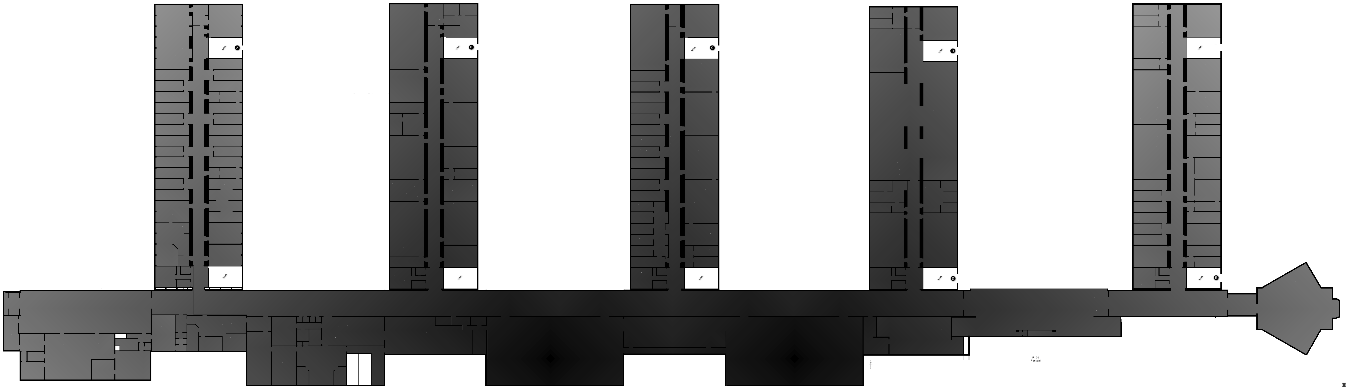
\includegraphics[scale=0.3]{img/wavefront_path.png}
\caption{How the wavefront expands from the two unloading--stations in the complete map.}
\label{fig::path}
\end{figure}

To control the order of the rooms to be cleared, has been made a graph consisting of sub--graphs, one for each block. Each room in a blok is connected to the center of the block, and each center of the blocks are connected to the closest unloading--station. To detect a room, the program has four steps
\begin{enumerate}\itemsep-3pt
\item First the upper left corners ($C_{ul}$) of the squares are detected. Each pixel in the map is checked with a 3x3--mask, shown in table \ref{tab::ul_mask}, which looks at the pixel neighbors are obstacles, which corresponds to a left corner. If the mask matches, then the pixel is marked as a $C_{ul}$ and the position for the pixel is stored in a list. 

\begin{table}[H]
\centering
\begin{tabular}{|l|l|l|}
\hline
0 & 0 & 0 \\ \hline
0 & P &   \\ \hline
0 &   &   \\ \hline
\end{tabular}
\caption{3x3 mask for detecting upper left corners}
\label{tab::ul_mask}
\end{table}

\item Next the upper right corners ($C_{ur}$) is found by taking the the position for each $C_{ul}$, and then keep moving to the right, until it hits an obstacle. When it hits an obstacle, the pixel just before is marked as a $C_{ur}$ and stored in a data type, called \lstinline|square|. On table \ref{tab::corner_detection} is this approach shown.
\item Next the lower left corners $C_{ll}$ is found, just like the $C_{ur}$, by taking the the position for each $C_{ul}$, but instead it keeps moving down, until it hits an obstacle. When it hits an obstacle, the pixel just before is marked as a $C_{ll}$ and stored in \lstinline|square|. On table \ref{tab::corner_detection} is this approach shown. 
\item The lower right corner ($C_{lr}$) is not detected like the other three corners, it is calculated by taking the height distance (in pixels) between $C_{ul}$ and $C_{ll}$, and assuming that the $C_{lr}$ has the same height distance from the $C_{ur}$. Like the other corners, the $C_{lr}$ is marked and stored in \lstinline|square|. 
\end{enumerate} 

\begin{table}[H]
\centering
\begin{tabular}{|c|
>{\columncolor[HTML]{C0C0C0}}c ccccccc|c|}
\hline
\cellcolor[HTML]{000000}{\color[HTML]{FFFFFF} 0} & \multicolumn{1}{l|}{\cellcolor[HTML]{000000}{\color[HTML]{FFFFFF} 0}} & \multicolumn{1}{l|}{\cellcolor[HTML]{000000}{\color[HTML]{FFFFFF} 0}} & \multicolumn{1}{l|}{}            & \multicolumn{1}{l|}{}            & \multicolumn{1}{l|}{}            & \multicolumn{1}{l|}{}            & \multicolumn{1}{l|}{}            &                                  &                                                  \\ \hline
\cellcolor[HTML]{000000}{\color[HTML]{FFFFFF} 0} & \cellcolor[HTML]{9B9B9B}$C_{ul}$                                      & \cellcolor[HTML]{C0C0C0}$\cdots$                                      & \cellcolor[HTML]{C0C0C0}$\cdots$ & \cellcolor[HTML]{C0C0C0}$\cdots$ & \cellcolor[HTML]{C0C0C0}$\cdots$ & \cellcolor[HTML]{C0C0C0}$\cdots$ & \cellcolor[HTML]{C0C0C0}$\cdots$ & \cellcolor[HTML]{9B9B9B}$C_{ur}$ & \cellcolor[HTML]{000000}{\color[HTML]{FFFFFF} 0} \\ \cline{1-1} \cline{10-10} 
\cellcolor[HTML]{000000}{\color[HTML]{FFFFFF} 0} & $\vdots$                                                              & \cellcolor[HTML]{C0C0C0}                                              & \cellcolor[HTML]{C0C0C0}         & \cellcolor[HTML]{C0C0C0}         & \cellcolor[HTML]{C0C0C0}         & \cellcolor[HTML]{C0C0C0}         & \cellcolor[HTML]{C0C0C0}         & \cellcolor[HTML]{C0C0C0}$\vdots$ &                                                  \\ \cline{1-1} \cline{10-10} 
                                                 & $\vdots$                                                              & \cellcolor[HTML]{C0C0C0}                                              & \cellcolor[HTML]{C0C0C0}         & \cellcolor[HTML]{C0C0C0}         & \cellcolor[HTML]{C0C0C0}         & \cellcolor[HTML]{C0C0C0}         & \cellcolor[HTML]{C0C0C0}         & \cellcolor[HTML]{C0C0C0}$\vdots$ &                                                  \\ \cline{1-1} \cline{10-10} 
                                                 & $\vdots$                                                              & \cellcolor[HTML]{C0C0C0}                                              & \cellcolor[HTML]{C0C0C0}         & \cellcolor[HTML]{C0C0C0}         & \cellcolor[HTML]{C0C0C0}         & \cellcolor[HTML]{C0C0C0}         & \cellcolor[HTML]{C0C0C0}         & \cellcolor[HTML]{C0C0C0}$\vdots$ &                                                  \\ \cline{1-1} \cline{10-10} 
{\color[HTML]{FFFFFF} $\cdots$}                  & $\vdots$                                                              & \cellcolor[HTML]{C0C0C0}                                              & \cellcolor[HTML]{C0C0C0}         & \cellcolor[HTML]{C0C0C0}         & \cellcolor[HTML]{C0C0C0}         & \cellcolor[HTML]{C0C0C0}         & \cellcolor[HTML]{C0C0C0}         & \cellcolor[HTML]{C0C0C0}$\vdots$ & {\color[HTML]{FFFFFF} $\cdots$}                  \\ \cline{1-1} \cline{10-10} 
                                                 & $\vdots$                                                              & \cellcolor[HTML]{C0C0C0}                                              & \cellcolor[HTML]{C0C0C0}         & \cellcolor[HTML]{C0C0C0}         & \cellcolor[HTML]{C0C0C0}         & \cellcolor[HTML]{C0C0C0}         & \cellcolor[HTML]{C0C0C0}         & \cellcolor[HTML]{C0C0C0}$\vdots$ &                                                  \\ \cline{1-1} \cline{10-10} 
                                                 & $\vdots$                                                              & \cellcolor[HTML]{C0C0C0}                                              & \cellcolor[HTML]{C0C0C0}         & \cellcolor[HTML]{C0C0C0}         & \cellcolor[HTML]{C0C0C0}         & \cellcolor[HTML]{C0C0C0}         & \cellcolor[HTML]{C0C0C0}         & \cellcolor[HTML]{C0C0C0}$\vdots$ &                                                  \\ \cline{1-1} \cline{10-10} 
                                                 & \cellcolor[HTML]{9B9B9B}$C_{ll}$                                      & \cellcolor[HTML]{C0C0C0}$\cdots$                                      & \cellcolor[HTML]{C0C0C0}$\cdots$ & \cellcolor[HTML]{C0C0C0}$\cdots$ & \cellcolor[HTML]{C0C0C0}$\cdots$ & \cellcolor[HTML]{C0C0C0}$\cdots$ & \cellcolor[HTML]{C0C0C0}$\cdots$ & \cellcolor[HTML]{9B9B9B}$C_{lr}$ &                                                  \\ \hline
                                                 & \multicolumn{1}{l|}{\cellcolor[HTML]{000000}{\color[HTML]{FFFFFF} 0}} & \multicolumn{1}{l|}{}                                                 & \multicolumn{1}{l|}{}            & \multicolumn{1}{l|}{}            & \multicolumn{1}{l|}{}            & \multicolumn{1}{l|}{}            & \multicolumn{1}{l|}{}            &                                  &                                                  \\ \hline
\end{tabular}
\caption{Detection of the room corners}
\label{tab::corner_detection}
\end{table}
\subsection{Results}
How long does it take?

\subsection{Conclusion}
What works and what does not? Why?
